\begin{figure}[!htbp]
    \vspace{-0.5em}
    \centering
    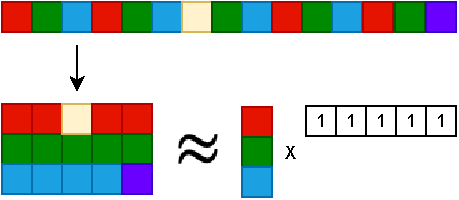
\includegraphics[width=0.3\textwidth]{\fighome/modularity.pdf}
    \vspace{-0.5em}
    \caption{\textbf{Tensor reshaping.} 
    The figure shows how reshaping can help reduce the number of parameters while preserving critical structural properties. A vector of length 15 displays periodicity in its entries (represented here by repeating colors) except for a few entries. Reshaping it into a $3\times 5$ matrix and then taking a factorized tensor approximation (rank-1 SVD) \textbf{a)} reduces the number of parameters to store and \textbf{b)} culls out artifacts (non-periodic elements) while representing periodicity sans redundancy.
    }
\label{fig:periodicity}
\vspace{-1em}
\end{figure}